   	\newpage
	\section{Implementierungen}

	Das folgende Kapitel der \textit{Implementierungen} gibt einen Überblick über die verwendeten Technologien für das Produkt. Es werden genutzte (offene) Schnittstellen genannt, vorgestellt und deren Funktionsweise beschrieben. Zusätzlich werden selbst entwickelte Komponenten beschrieben und deren Implementierungen (sofern nötig) erörtert.
	
	\subsection{Arduino}
	
	Die Arduinoplattform ermöglicht eine \texttt{stackable}\footnote{aufeinderstecken verschiedener Module - vergleichbar mit Lego-Prinzip} Aneinanderkopplung verschiedener technischer Module. Unter anderem wurden in diesem Projekt ein e-Health-Modul, zum Auslesen von Galvanic Skin Daten, und zum Anderen die Anbindung an ein Wireless + Bluetooth Shield verwandt und eingesetzt. Die einzelnen Komponeten werden wie folgt beschrieben und durch die Beschreibung des Endprodukts vervollständigt.
		
	\subsubsection{eHealth - Plattform}
	
	Das e-Health-Modul ermöglicht es Android-Nutzer auf biometrische Daten zuzugreifen. Zu diesen Daten zählen unter anderem Puls-Messung, Blutdruck, EKG, Kör-pertemperatur und auch die Hautleitfähigkeit (GSR \^= galvanic skin response).

	Das e-Helath-Modul ist stackable und lässt sich daher einfach auf ein Arduino Uno ,,aufsetzen``. Hier ist darauf zu achten, dass es nicht zu verbogenen oder abgebrochenen Metall- / Verbindungsstücken kommt.
	
	\begin{figure}[hbtp]
	\centering
	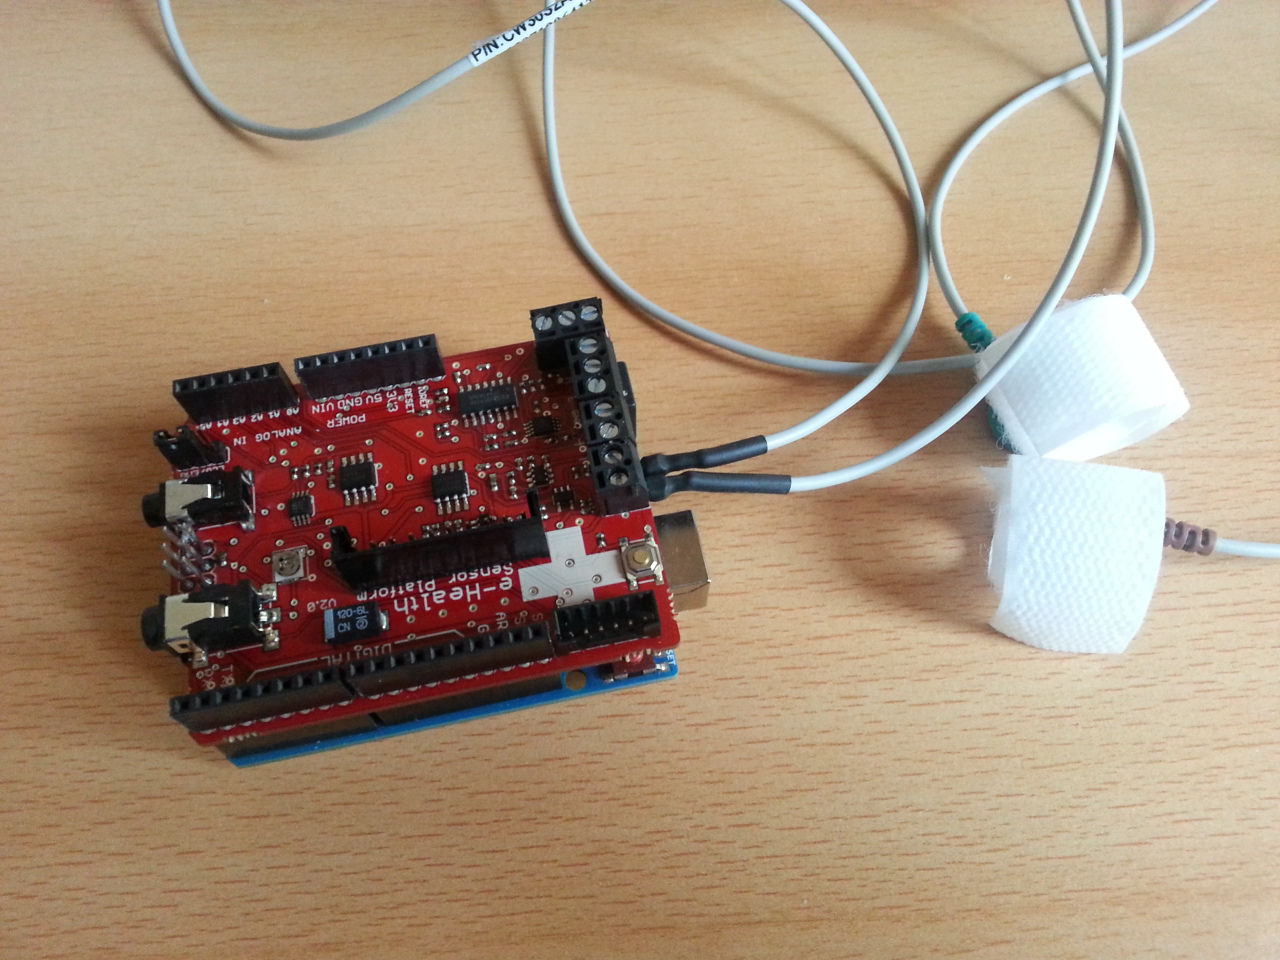
\includegraphics[width=0.7\textwidth]{implementierung_arduino+ehelath-modul.jpg}
	\caption{Arduino-eHealth-Stack}
	\label{fig:Arduino-eHealth-Stack}
	\end{figure}
	
	
	Zur Programmierung eines Arduino-Programms ist neben der Installation der entsprechenden Arduino IDE und der Treiberinstallation der Arduino Hardware, die entsprechenden e-Health Libraries herunterzuladen und unter dem Standardinstallationsordner der Arduino-IDE abzulegen, z.B.:
	\begin{itemize}
	\item \texttt{C:\textbackslash Arduino\textbackslash arduino-1.0.5\textbackslash libraries\textbackslash eHealth}
	\item \texttt{C:\textbackslash Arduino\textbackslash arduino-1.0.5\textbackslash libraries\textbackslash PinChangeInt}
	\end{itemize}
	
	Danach kann in der Arduino IDE das gewünschte Programm erstellt werden. Dazu sollte zuerst das e-Health Package eingebunden werden, dann kann man auf den / die gewünschten Sensor / -en zugreifen:
	
	\begin{enumerate}
	 \item \texttt{\#include $ <eHealth.h> $}
	 \item ...
	 \item \texttt{float resistance = $eHealth$.getSkinResistance();}
	 \end{enumerate} 
	 
	 Die Variable $resistance$ sollte in der loop-Funktion deklariert und definiert werden, um sicher zu stellen, dass die Werte immer ,,frisch`` in die Variable geschrieben werden.
	 
	 Für weitere Information zur e-Health-Plattform im besonderen zur GSR verweisen wir auf die \href{http://www.cooking-hacks.com/documentation/tutorials/ehealth-biometric-sensor-platform-arduino-raspberry-pi-medical\#step4\_7}{e-Health-Website}.
	
	\subsubsection{Wireless + Bluetooth Shield}
	
	Das Wireless + Bluetooth Shield es ebenfalls stackable und kann auf das Arduino Uno aufgesetzt werden. 
	Im folgenden Fall stand neben dem Wireless Shield das Zusatzmodul \texttt{BlueTooth Bee} von iteadstudio zur Verfügung. Das Bluetooth-Modul hatte die Spezifikation V2.0 und Modelbezeichnung HC-06. 
	
		\begin{figure}[hbtp]
		\centering
		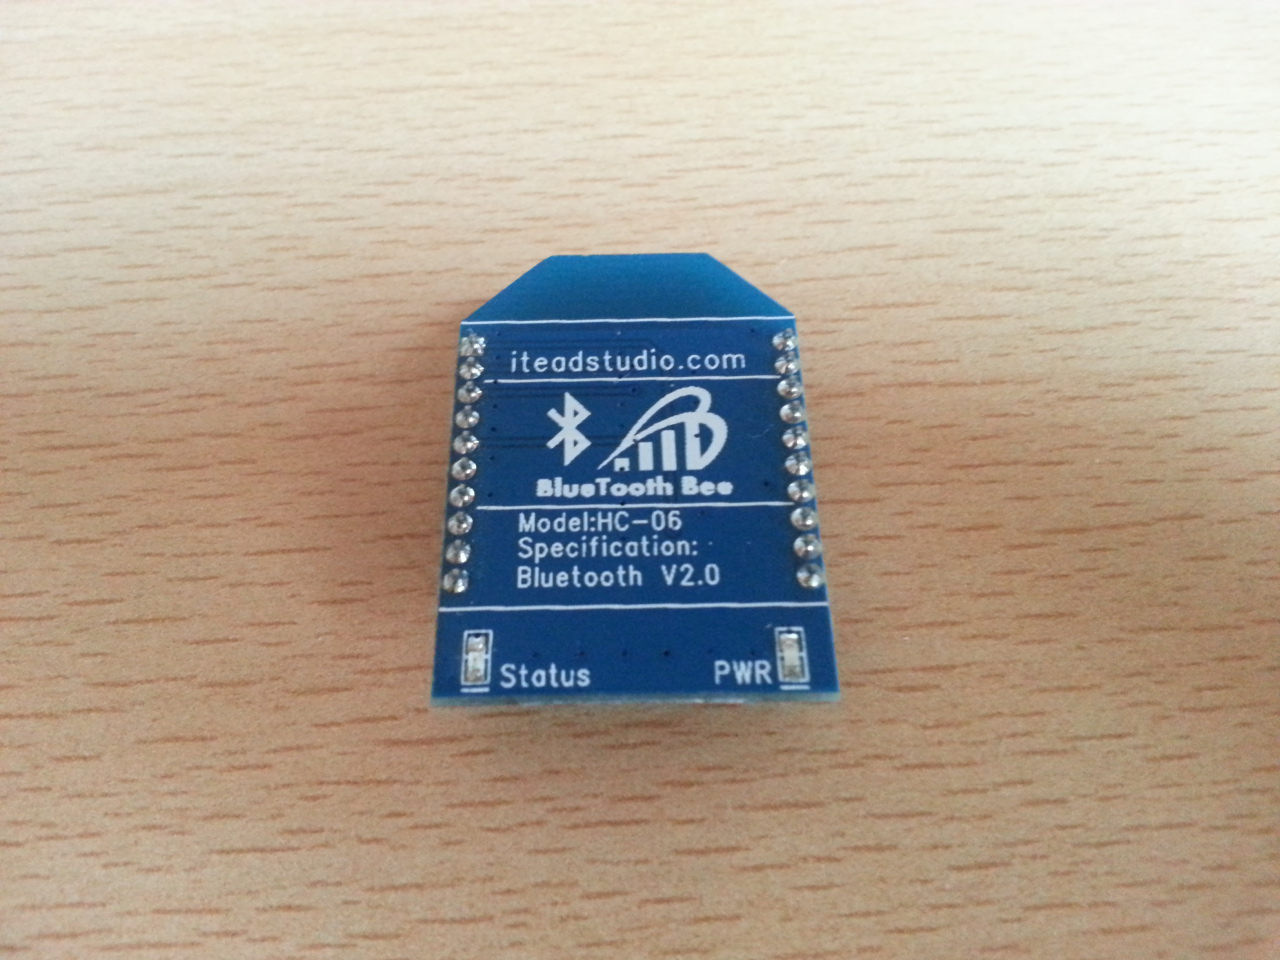
\includegraphics[width=0.7\textwidth]{implementierung_bluetooth-modul.jpg}
		\caption{Das Bluetooth Modul}
		\label{fig:Bluetooth-Modul}
		\end{figure}
		
	
	Die Modelbezeichnung ist ausschlaggebend dafür, ob ein solches Modul im Master\footnote{kann aktives Pairing zu anderen Geräten übernehmen (Serverfunktionalität)}, Master+Slave oder nur Slave\footnote{kann kein Pairing übernehmen} Modus arbeitet. In diesem Fall bestand mit diesem Modul die einfache Slave-Funktionalität zur Verfügung.
	
	\begin{figure}[hbtp]
	\centering
	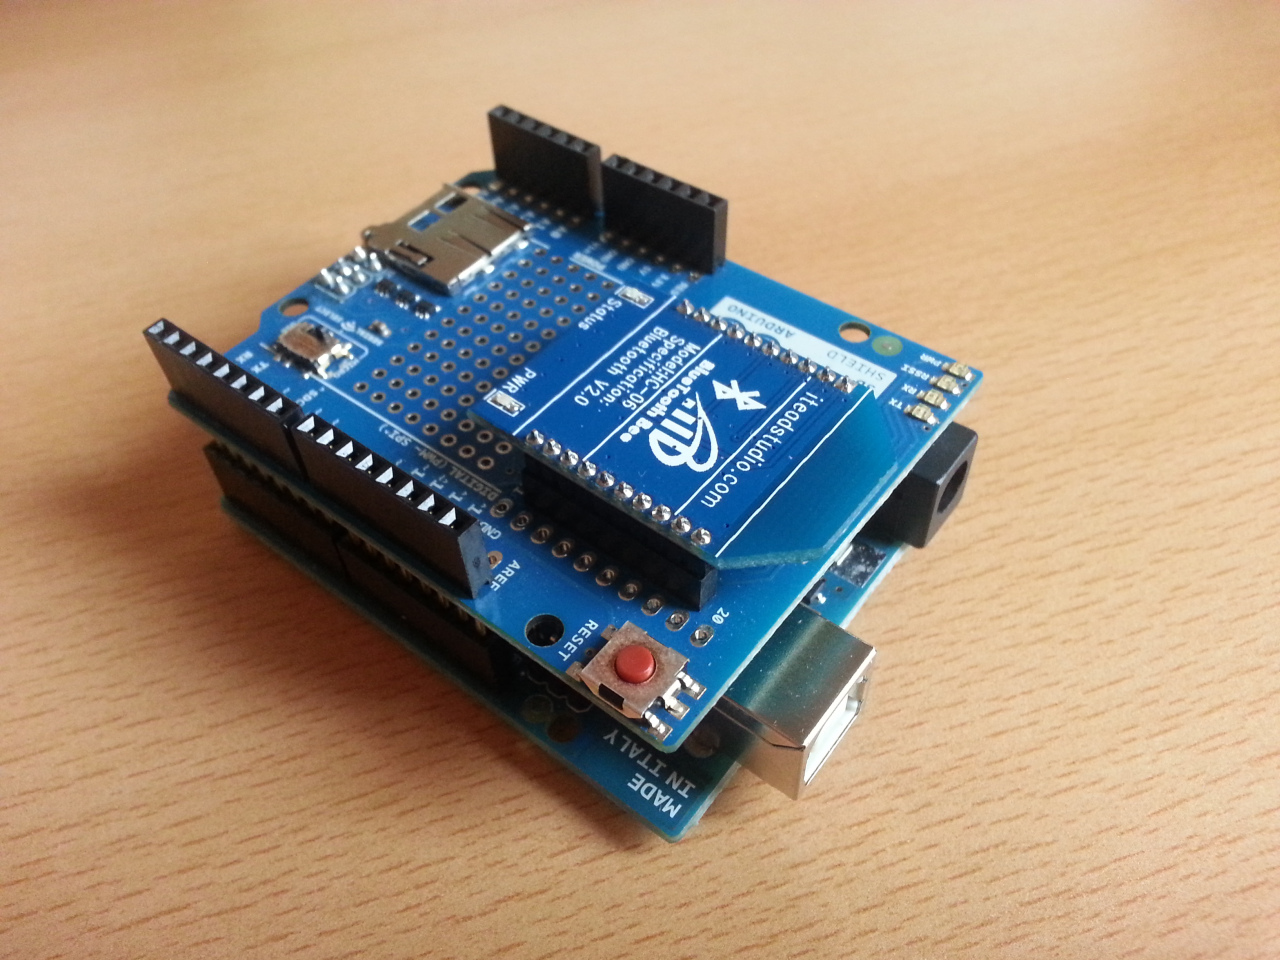
\includegraphics[width=0.7\textwidth]{implementierung_arduino+wireless-shield.jpg}
	\caption{Der Ardunio-Bluetooth-Stack}
	\label{fig:Arduino-Bluetooth-Stack}
	\end{figure}
	
	Die Implementierung der Bluetooth-Verbindung läuft im Slave-Modus über die serielle Verbindung. Dazu wird im Setup ein \texttt{Serial.begin($<baud\_rate>$)} aufgerufen. Die Baudrate richtet sich nach der Übertragungsgeschwindigkeit mit der das Bluetooth-Modul arbeiten soll und mit der die entsprechende Gegenstation (Master) arbeitet. 
	
	In der $loop()$-Funktion ist dann der entsprechende zu übertragende Wert mit \\$Serial.print(<value>)$ über die serielle Schnittstelle auszugeben. Zusätzlich ist nach jedem Wert die Zeichnkette ,,\textbackslash r\textbackslash n'' mit $Serial.print();$ zu übergeben. Sie signalisiert den Abschluss eines Datensatzes.
	
	
	\subsubsection{Endprodukt}

	Beim Zusammenfügen der einzelnen Komponenten musste die Reihenfolge:
	\begin{itemize}
	\item Oben: Wireless + Bluetooth - Shield
	\item Mitte: e-Health-Modul
	\item Unten: Arduino Uno
	\end{itemize}
	
	eingehalten werden, da sonst das e-Health-Modul nicht mit Strom versorgt wird, wenn Wireless und e-Health miteinander getauscht werden. 
	
	\begin{figure}[hbtp]
	\centering
	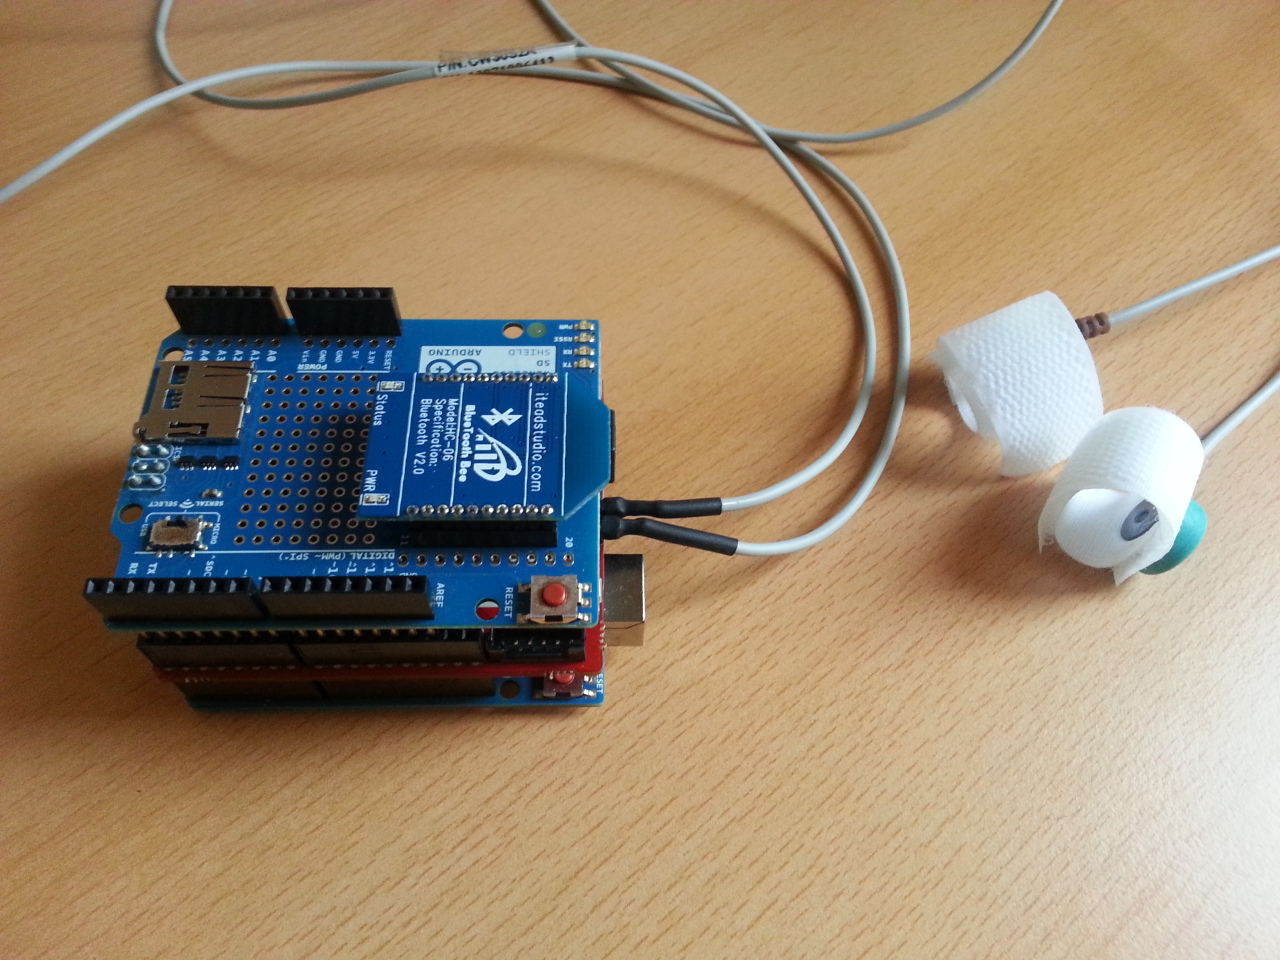
\includegraphics[width=0.7\textwidth]{implementierung_completestack.jpg}
	\caption{Der vollständige Stack}
	\label{fig:completeStack}
	\end{figure}
	
	
	\newpage
	\subsection{Android}
	
	Bei der Android-Entwicklung wurde auf eine Unterstützung mit \texttt{git} entwickelt. So konnte der Quellcode sowohl für Android- als auch Arduino- und LaTex-Quellcode versioniert verwaltet werden.
	
	\subsubsection{EEG: NeuroSky Brainwave Headset}
	
	Um das NeuroSky EEG Headset in Android anbinden zu können, bedarf es einiger Vorbereitungen:
	\begin{enumerate}
	\item Kauf und Download des Developer Tool für Android vom \href{http://store.neurosky.com/products/developer-tools-3-android} {NeuroSky Store}
	\item Erzeugen eines \texttt{lib}-Ordners im Android-Projekt, sofern nicht schon vorhanden
	\item Ablegen der \texttt{ThinkGear.jar}-Datei im lib-Ordner
	\item Importanweisung: ,,\texttt{import com.neurosky.thinkgear.*;}`` in der entsprechenden Activity
	\item AndroidManifest.xml: es ist die Bluetooth\_Permission zu setzen
	\end{enumerate}
	
	Des Weiteren müssen ein Android-BluetoothAdapter und ein TGDevice instanziiert werden.

	Der bluetoothAdapter wird mittels $BluetoothAdapter.getDefaultAdapter()$ zugewiesen. Wenn dieses erfolgreich war, dann wird das tgDevice erzeugt: $tgDevice = new TGDevice(bluetoothAdapter, handler);$. Dem tgDevice wird der Default-BluetoothAdapter und eine $handler$ zugewiesen. 
	
	Der handler \label{handler} wird einer Handler-Class erzeugt. Dieser $handler$ hat die Aufgabe, Daten, die das Gerät sendet abzufangen und in einer gewünschten Form zu verarbeiten. Exemplarisch für die Aufmerksamkeitswerte des EEG:
	
	\begin{enumerate}
	\item case TGDevice.MSG\_ATTENTION:
    \item eeg\_att.setText('' Attention: " + msg.arg1 + "\textbackslash n" + eeg\_att.getText());
	\item break;
	\end{enumerate}
	
	Folgende Daten können vom EEG ausgelesen werden:
	
	\begin{itemize}
	\item Verbindungsstatus: STATE\_CONNECTING, STATE\_CONNECTED, \\STATE\_NOT\_FOUND, STATE\_NOTE\_PAIRED, STATE\_DISCONNECTED
	\item Auslesedaten: MSG\_ATTENTION, MSG\_Meditation, MSG\_BLINK, \\MSG\_HEART\_RATE
	\item sonstige Status: MSG\_LOW\_BATTERY, MSG\_POOR\_SIGNAL
	\end{itemize}
	
	Entscheidend für den Lügendetektor sind die Werte aus MSG\_ATTENTION, \\MSG\_MEDITATION und MSG\_BLINK. Anhand der Aufmerksamkeits- (attention) und Ruhewerte (meditation) kann man die Aufregung bzw. Entspannung bei der Testperson ablesen. Hinzu kommen die Augenblinzler (blink), die stark oder schwach ausgeprägt sein bzw. gezählt werden können und daher auf zusätzliches ,,unkontrolliertes`` / ,,nervöses`` Verhalten hinweisen.
	
	\begin{figure}[h!btp]
	\centering
	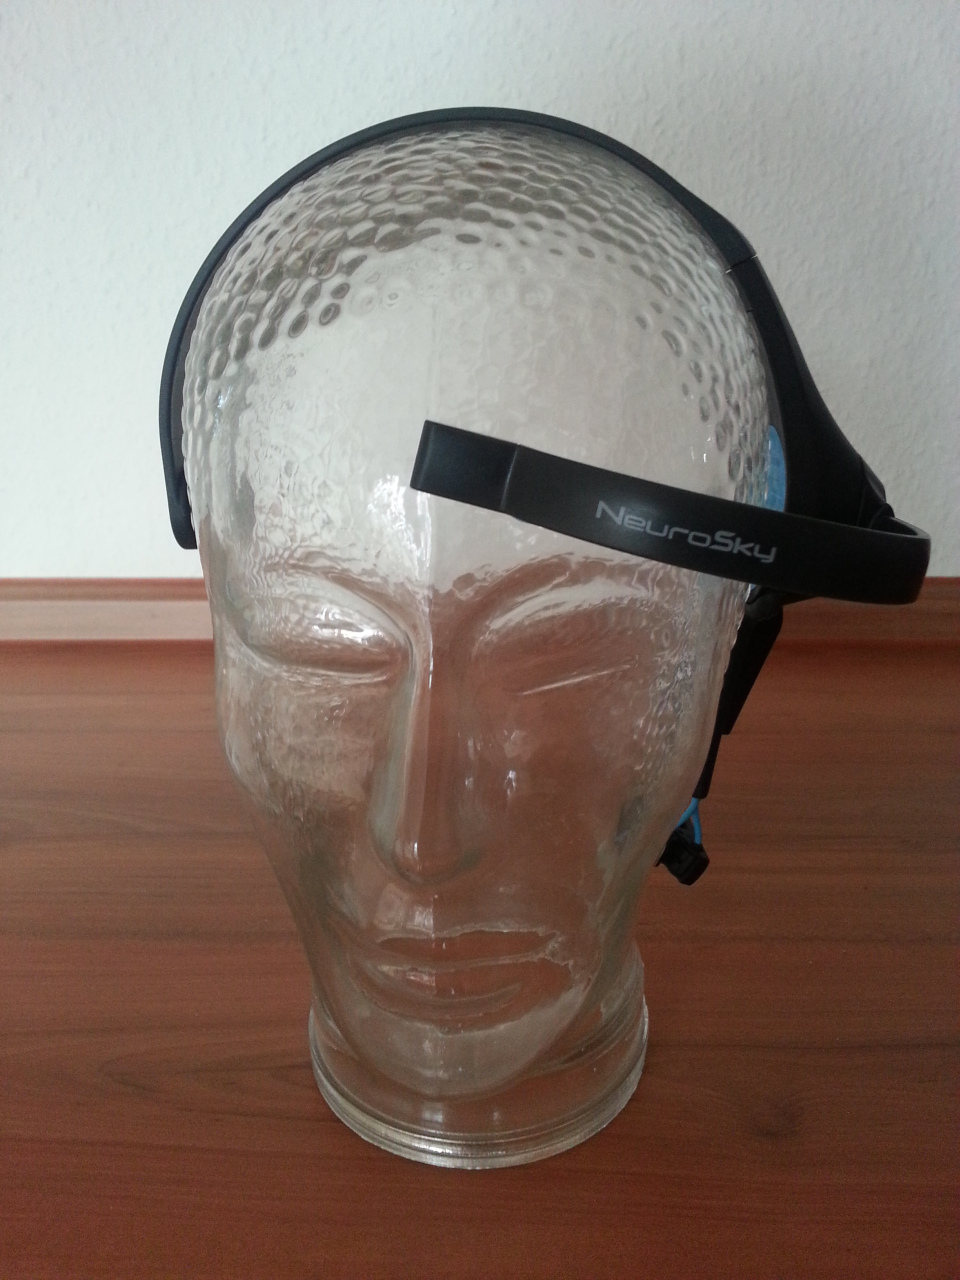
\includegraphics[width=0.5\textwidth]{implementierung_neuroskyheadset.jpg}
	\caption{Das NeuroSky Brainwave Headset}
	\label{fig:Brainwave-Headset}
	\end{figure}
	
	Das Anbinden des EEG an die Android-Applikation erfolgt über Bluetooth. Vor dem ersten Starten der Anwendung sollte das Android-Gerät mit dem EEG gepairt werden. Dann kann die eigene Anwendung gestartet werden. Sollte keine Verbindung in der Anwendung angezeigt werden, so sollte zusätzlich auf der EEG-Rückseite der ,,Pairing``-Knopf gedrückt werden.
	
	\subsubsection{Arduino Bluetooth}
			
	Zur Anbindung des Arduino Bluetooth Moduls kann man zweierlei vorgehen:
	\begin{enumerate}
	\item automatisierter (statischer) Verbindungsaufbau zwischen Android und Arduino
	\item dynamischer Verbindungsaufbau durch scannen vorhandener Bluetooth-Geräte
	\end{enumerate}
	
	Wir haben uns im Projekt dazu entschieden, dass wir die statische Methode wählen, da über das Scannen vorhandener Geräte der Verbindungsaufbau zu Fehlverbindungen geführt hatte und ggf. die Applikation geschlossen bzw. die built-in Bluetooth Funktionalität neugestartet werden musste. 
	
	Um die automatisierte Verbindung zu realisieren mussten eineige Vorbedingungen erfüllt werden:
	\begin{itemize}
	\item MAC-Adresse des Bluetooth-Moduls scannen
	\item MAC-Adresse in der Applikation hinterlegen
	\item SPP\footnote{serial port profile} UUID\footnote{128-bit universally unique identifier} für Verbindung festlegen\footnote{wird für Bluetooth Socket benötigt}
	\end{itemize}
	
	Zur Identifizierung des Arduino Bluetooth Moduls ,,linvor`` konnten wir mit der App $Power Bluetooth Scanner$ die MAC-Adresse ,,00:12:07:17:18:24`` auslesen. 
	Beim Aufbau der Bluetooth Verbindung soll eine UUID hinterlegt werden. Android (Google Inc.) selbst schlägt vor: ,,If you are connecting to a Bluetooth serial board then try using the well-known SPP UUID 00001101-0000-1000-8000-00805F9B34FB.``\footnote{http://developer.android.com/reference/android/bluetooth/BluetoothDevice.html}. 
	Auch für die Arduino Bluetooth zu Android Verbindung muss ein Handler erzeugt werden (vgl. EEg-handler auf Seite \pageref{handler}).
	In diesem Fall musste der eingehende Datenstrom in ein byte-Array umgewandelt werden: $byte[] readBuf = (byte[]) msg.obj;$. Ausgehend von dem $msg.obj$ das über die seriellen Schnittstelle übertragen wird, können diese Signale in ein byte-Array gecastet und der Variable $readBuf$ zugewiesen werden. Aus dem byte-Array kann dann mittels $new String()$ ein String erzeugt und weiter verarbeitet werden.
	
	Die eigentliche Bluetooth-Verbindung wird in der $onResume()$ Methode hergestellt. Hierzu wird einer Variable btAdapter (von BluetoothAdapter, siehe EEG) durch die Methode $create BluetoothSocket(device)$ gesetzt. 
	Der Parameter device ist eben die Verbindung (über die MAC-Adresse) zum Ardunio Bluetooth Shield \\ \\
	$BluetoothDevice$ $device = btAdapter.getRemoteDevice(ADDRESS);$\\ \\
	Mit der Erstellung des Bluetooth-Socket kann nun ein Verbindungs-Thread (ConnectedThread) erzeugt werden. Dieser sorgt dafür, dass die eingehenden Daten ordnungsgemäß (ge'threaded') empfangen (wenn gewünscht auch gesendet) werden können. 
	
	Mit $mConnectedThread = new ConnectedThread(btSocket);$ und \\$mConnectedThread.start();$ wird der Thread gestartet.
	
	\subsubsection*{Bluetooth-Status überprüfen}
	
	Da eine gültige Verbindung nur mit angeschaltetem Bluetooth-Modul des mobilen Geräts funktioniert, muss von der Anwendung überprüft werden, ob Bluetooth angeschaltet ist. Dazu wird die Methode \texttt{checkBTState()} genutzt. Sie wird in der Activity-Methode \texttt{onCreate()} gestartet und überprüft folgende Status:
	\begin{enumerate}
	\item wurde ein Bluetooth-Adapter angelegt, wenn nicht, dann beende und gib Fehlermeldung aus
	\item Bluetooth-Adapter vorhanden und ,,enabled``, dann ist alles ok
	\item Bluetooth-Adapter vorhanden aber nicht ,,enabled``, dann erzeuge und rufe einen Intent mit $BluetoothAdapter.ACTION\_REQUEST\_ENABLE$ auf und starte die Methode $startActivityForResult()$ um das Anschalten des Bluetooth-Mo-duls zu erzwingen.
	\end{enumerate}
	
	\subsubsection{Spielaufbau}
	
	
	\subsubsection{Datenpersistenz}
	
	
	\subsubsection{Datenvisualisierung}
